\begin{frame}[hasprev=false, hasnext=true]
\label{example:mars-pathfinder}
\frametitle{Mars Pathfinder}
\framesubtitle{Description}

\begin{itemize}
	\item Mars Pathfinder was a low-cost planetary mission to Mars
	\begin{itemize}
		\item Landed on Martian surface at July 4th, 1997.
	\end{itemize}

	\item It demonstrated several new technologies for Mars exploration:
	\begin{itemize}
		\item Airbag-based landing mechanism.
		\item Use of rovers to collect and analyse soil and rock samples.
	\end{itemize}

	\item The spacecraft had two parts: the lander and the rover.
\end{itemize}

\begin{figure}
	\centering
	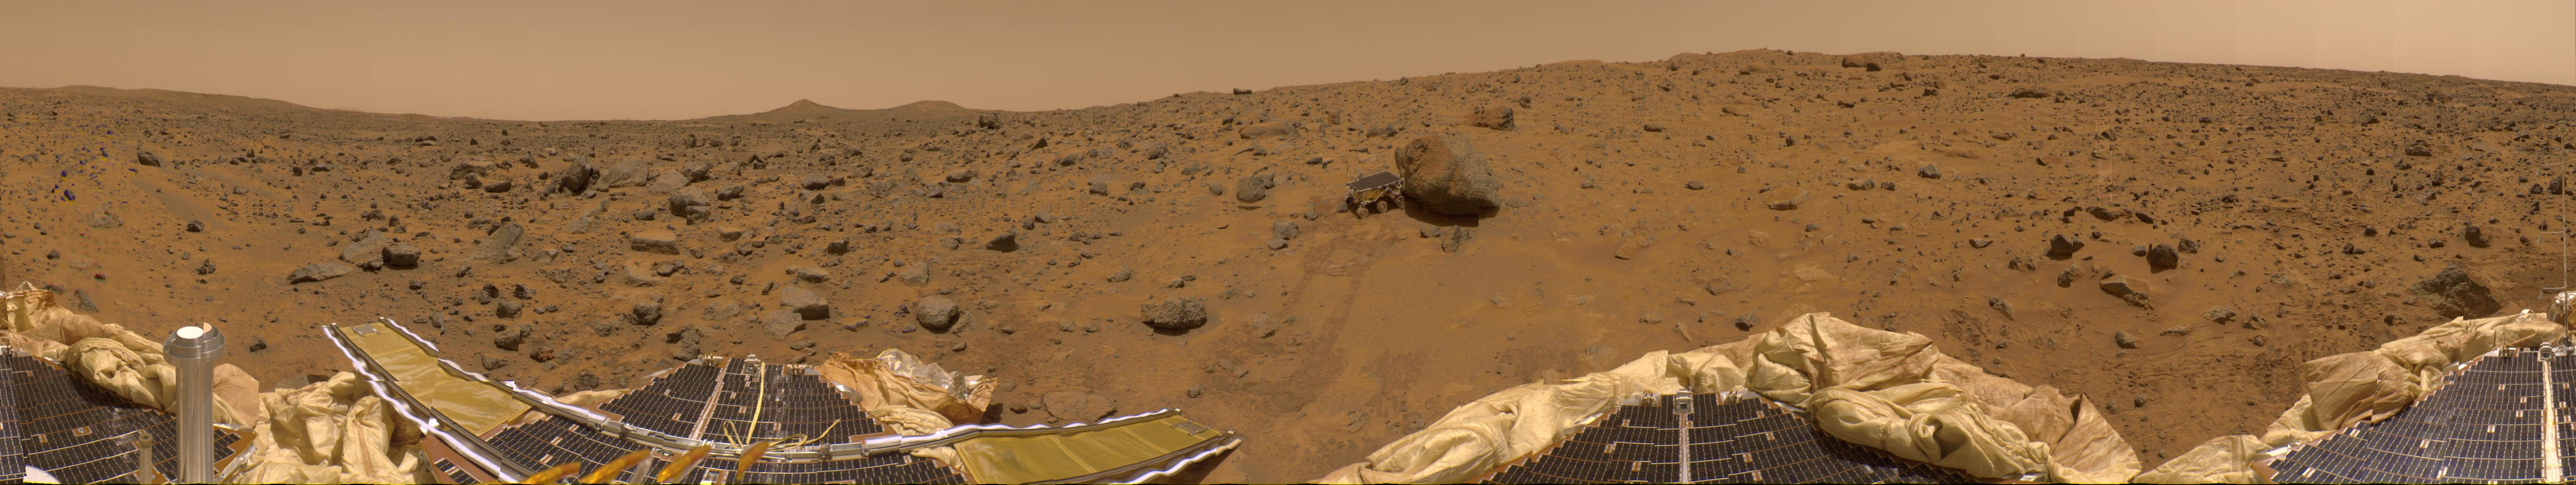
\includegraphics[width=\textwidth]{aux/examples/mars-pathfinder/mars-pathfinder}
\end{figure}
\end{frame}


\begin{frame}[hasprev=true, hasnext=true]
\frametitle{Mars Pathfinder}
\framesubtitle{Problem}

\begin{itemize}
	\item After collecting data for a long period, the lander would reset
	itself and all the data was lost.
\end{itemize}

\begin{figure}
	\centering
	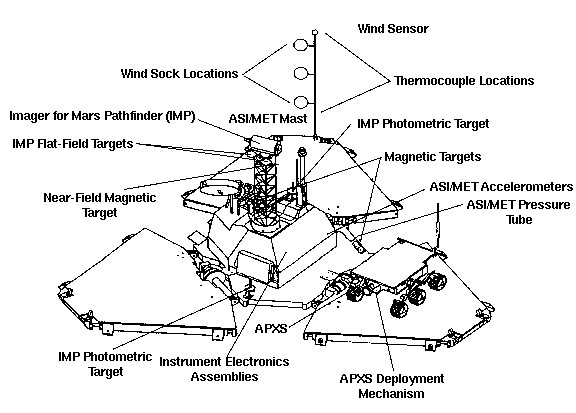
\includegraphics[width=7.5cm]{aux/examples/mars-pathfinder/mars-pathfinder-lander}
\end{figure}
\end{frame}


\begin{frame}
\frametitle{Mars Pathfinder}
\framesubtitle{Diagnostic}

\begin{itemize}
	\item The lander software was concurrent and employed preemptive
	scheduling.

	\item Each thread had a priority and exchanged information between each
	other using an information bus.
	\begin{itemize}
		\item Information bus = shared memory which access was controlled
		by a mutex.
	\end{itemize}

	\item The information bus management system itself was a thread that
	run frequently, with a high priority.

	\item Another applications that run in the system was:
	\begin{itemize}
		\item meteorological system, run much less frequently and with lower
		priority, and

		\item communication thread: medium priority, but run frequently.
	\end{itemize}
\end{itemize}
\end{frame}



\begin{frame}
\frametitle{Mars Pathfinder}
\framesubtitle{Diagnostic}

\begin{itemize}
	\item This combination of threads \textbf{usually} worked correctly.

	\item However, the information bus management system could be blocked
	in the mutex in the following situation:
	\begin{enumerate}
		\item Communication thread is scheduled and uses the processor, as
		it has higher priority than the meteorological thread.

		\item Communication thread can take as much time as it needs to
		run.

		\item However, a timer is expired whenever the information bus
		thread is not executed for a long time.

		\item The corrective measure taken by the timer is to reset the
		system.
	\end{enumerate}
\end{itemize}
\end{frame}



\begin{frame}[hasprev=true, hasnext=false]
\frametitle{Mars Pathfinder}
\framesubtitle{Solution}

\begin{itemize}
	\item Change the value of a constant in the software, enabling priority
	inheritance.
	\begin{itemize}
		\item When the information bus was blocked in the mutex, the
		meteorological thread would heritage the information bus thread
		priority, thus avoiding the communication thread to run for a too
		long time.
	\end{itemize}
\end{itemize}

\begin{figure}
	\centering
	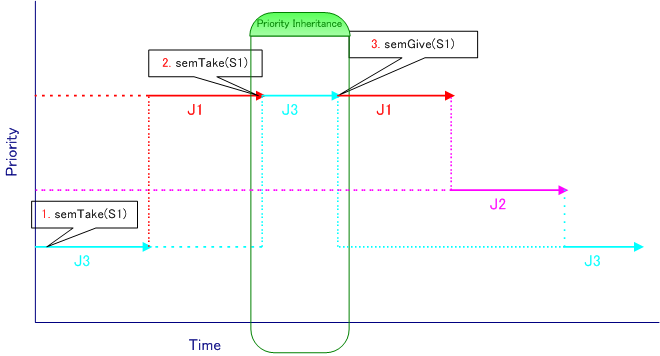
\includegraphics[width=4cm]{aux/examples/mars-pathfinder/priority-inheritance}
	\caption{Priority inheritance example.}
\end{figure}

\end{frame}